\documentclass{article}
\usepackage{graphicx}
\usepackage[lithuanian]{babel}
\usepackage{amsmath}
\usepackage[utf8]{inputenc}
\usepackage[T1]{fontenc}
\usepackage{lmodern}
\usepackage{mathtools}
\usepackage{tikz}

\title{Kvantiniai skaičiavimai}
\author{Adrian Klimaševski}
\date{2025 m. rugsėjis}

\begin{document}

\maketitle

\section*{Kompleksiniai skaičiai}

\textbf{1.} Apskaičiuokite reiškinių reikšmes. Būtinai parodykite tarpinius skaičiavimus:

\begin{align}
\text{1)}\quad &(2-2i)^{-2} + \frac{6-3i}{2-2i} + \frac{6+3i}{1+i}\nonumber
\end{align}

\text{Sprendimas:}

\begin{equation}
\frac{1}{(2-2i)^2} + \frac{(6-3i) \cdot (1+i)}{2(1-i) \cdot (1+i)} + \frac{(6+3i) \cdot 2(1-i)}{(1+i) \cdot 2(1-i)}\tag{1}
\end{equation}

\begin{equation}
\frac{1}{4-8i+4i^2} + \frac{6+3i-3i^2}{2-2i^2} + \frac{12-6i-6i^2}{2-2i^2}\tag{2}
\end{equation}

\begin{equation}
\frac{1 \cdot (-i)}{-8i \cdot (-i)} + \frac{9+3i}{4} + \frac{18-6i}{4}\tag{3}
\end{equation}

\begin{equation}
\frac{i}{8} + \frac{27-3i}{4}\tag{4}
\end{equation}

\begin{equation}
\frac{i}{8} + \frac{(27-3i) \cdot 2}{4 \cdot 2}\tag{5}
\end{equation}

\begin{equation}
\frac{i}{8} + \frac{54-6i}{8}\tag{6}
\end{equation}

\begin{equation}
\frac{54-5i}{8}\tag{7}
\end{equation}

\begin{equation}
\frac{54}{8}+\frac{5}{8}i\tag{8}
\end{equation}

\text{Atsakymas:}
\begin{equation*}
\frac{27}{4}+\frac{5}{8}i
\end{equation*}


\textbf{2.} Tarkime, kad
\begin{align*}
    u_1&=3+3i,\\
    w&=2-2i,\\
    z&=4+2i.
\end{align*}Apskaičiuokite reiškinių reikšmes. Būtinai parodykite tarpinius skaičiavimus:

\begin{align}
\text{1)}\quad & |u|+\overline{w}+\frac{z}{|z+1|}\nonumber
\end{align}

\text{Sprendimas:}

\begin{equation}
|3+3i|+\overline{2-2i}+\frac{4+2i}{|4+2i+1|}\tag{1}
\end{equation}

\begin{equation}
|3+3i|+\overline{2-2i}+\frac{4+2i}{|5+2i|}\tag{2}
\end{equation}

\begin{equation}
\sqrt{3^2+3^2}+(2+2i)+\frac{4+2i}{\sqrt{5^2+2^2}}\tag{3}
\end{equation}

\begin{equation}
3\sqrt{2}+2+2i+\frac{4+2i}{\sqrt{29}}\tag{4}
\end{equation}

\begin{equation}
3\sqrt{2}+2+2i+\frac{(4+2i) \cdot \sqrt{29}}{\sqrt{29} \cdot \sqrt{29}}\tag{5}
\end{equation}

\begin{equation}
3\sqrt{2}+2+2i+\frac{4\sqrt{29}+2\sqrt{29}i}{29}\tag{6}
\end{equation}

\begin{equation}
3\sqrt{2}+2+2i+\frac{4\sqrt{29}}{29}+\frac{2\sqrt{29}i}{29}\tag{7}
\end{equation}

\text{Atsakymas:}
\begin{equation*}
(3\sqrt{2}+2+\frac{4\sqrt{29}}{29})+i(2+\frac{2\sqrt{29}}{29})
\end{equation*}


\pagebreak 

\textbf{3.} Užrašykite kompleksinius skaičius trigonometrinėje formoje (\(\rho e^{i \theta}\)). Būtinai parodykite tarpinius skaičiavimus:

\begin{align}
\text{1)}-\frac{50}{2}+\frac{50\sqrt{3}}{2}i \nonumber
\end{align}

\text{Sprendimas:}

\begin{equation}
-25+25\sqrt{3}i\tag{1}
\end{equation}

\begin{equation}
\rho=|z|=\sqrt{x^2+y^2}=\sqrt{(-25)^2+(25\sqrt{3})^2}=50\tag{2}
\end{equation}

\begin{equation}
\cos \theta = \frac{x}{|z|} = \frac{-25}{50} = -\frac{1}{2} \tag{3}
\end{equation}

\begin{equation}
\theta = \arccos(-\frac{1}{2}) = \frac{2\pi}{3} \tag{4}
\end{equation}

\text{Atsakymas:}

\begin{equation*}
50e^{i\frac{2\pi}{3}}
\end{equation*}

\pagebreak

\textbf{4.} Išspręskite lygtis (detaliai pateikdami sprendimą):

\begin{align}
\text{1)}\quad & 2x^2- 2x+10=0 \nonumber
\end{align}

\text{Sprendimas:}

\begin{equation}
2x^2- 2x+10=0\quad | :2 \tag{1}
\end{equation}

\begin{equation}
x^2- x+5=0\tag{2}
\end{equation}

\begin{equation}
D=(-1)^2-4 \cdot 1 \cdot 5=-19 \tag{3}
\end{equation}

\begin{equation}
\sqrt{D}=\sqrt{-19}=\sqrt{19} \cdot \sqrt{-1}=\sqrt{19}i\tag{4}
\end{equation}

\begin{equation}
x_{1,2}=\frac{1\pm\sqrt{19}i}{2}\tag{5}
\end{equation}

\text{Atsakymas:}

\begin{equation*}
x_{1}=\frac{1}{2}+\frac{\sqrt{19}}{2}i, \quad x_{2}=\frac{1}{2}-\frac{\sqrt{19}}{2}i
\end{equation*}


\pagebreak



\textbf{5.} Raskite skaičiaus \textit{z} visas \textit{n} - tosios šaknies reikšmes (Jūs turite pateikti tikslias reikšmes (su radikalais)):

\begin{align}
\text{1)}\quad & n=6,\quad z=-128; \nonumber
\end{align}

\text{Sprendimas:}

\begin{equation}
\rho=|z|=|-128|=128 \tag{1} 
\end{equation}

\begin{equation}
cos\theta = \frac{x}{|z|}=\frac{-128}{128}=-1 \tag{2} 
\end{equation}

\begin{equation}
\theta=\arccos(-1)=\pi\tag{3} 
\end{equation}

\vspace{5mm}
\text{Bendroji $n$-tosios šaknies ($n=6$) formulė:}

\[
w_k = \sqrt[6]{128}\, e^{i\frac{\pi+2k\pi}{6}}
= 2^{7/6}\left(\cos\frac{\pi+2k\pi}{6}+i\sin\frac{\pi+2k\pi}{6}\right), 
\quad k=0,1,\dots,5.
\]
\vspace{3mm}

\text{Visos šaknys:}
\[
\begin{aligned}
w_0 &= 2^{7/6}\left(\cos\frac{\pi}{6}+i\sin\frac{\pi}{6}\right) 
= 2^{7/6}\left(\tfrac{\sqrt{3}}{2}+i\tfrac{1}{2}\right)
= 2^{1/6}(\sqrt{3}+i), \\[6pt]
w_1 &= 2^{7/6}\left(\cos\frac{\pi}{2}+i\sin\frac{\pi}{2}\right) 
= i\,2^{7/6}, \\[6pt]
w_2 &= 2^{7/6}\left(\cos\frac{5\pi}{6}+i\sin\frac{5\pi}{6}\right) 
= 2^{7/6}\left(-\tfrac{\sqrt{3}}{2}+i\tfrac{1}{2}\right)
= 2^{1/6}(-\sqrt{3}+i), \\[6pt]
w_3 &= 2^{7/6}\left(\cos\frac{7\pi}{6}+i\sin\frac{7\pi}{6}\right) 
= 2^{7/6}\left(-\tfrac{\sqrt{3}}{2}-i\tfrac{1}{2}\right)
= 2^{1/6}(-\sqrt{3}-i), \\[6pt]
w_4 &= 2^{7/6}\left(\cos\frac{3\pi}{2}+i\sin\frac{3\pi}{2}\right) 
= -i\,2^{7/6}, \\[6pt]
w_5 &= 2^{7/6}\left(\cos\frac{11\pi}{6}+i\sin\frac{11\pi}{6}\right) 
= 2^{7/6}\left(\tfrac{\sqrt{3}}{2}-i\tfrac{1}{2}\right)
= 2^{1/6}(\sqrt{3}-i).
\end{aligned}
\]

\pagebreak

\textbf{6.} Nubraižykite sritį kompleksinėje plokštumoje, kurią atitinka visi skaičiai  \textit{z}, kurie tenkina sąlygas:

\begin{align}
\text{1)}\quad & 1 \leq |z-5| \leq 10,\quad \Re(z)>1;\nonumber
\end{align} 

\text{Sprendimas:}

\begin{equation}
-10 \leq z-5 \leq -1\quad| + 5
\end{equation}

\begin{equation}
-5 \leq z \leq 4
\end{equation}

\begin{equation}
1 \leq z-5 \leq 10\quad|+ 5
\end{equation}

\begin{equation}
6 \leq z \leq 15
\end{equation}

\vspace{7mm}
\centering{\textbf{Sritis:} $1\le |z-5|\le 10,\ \Re (z)>1$}\\
\vspace{5mm}

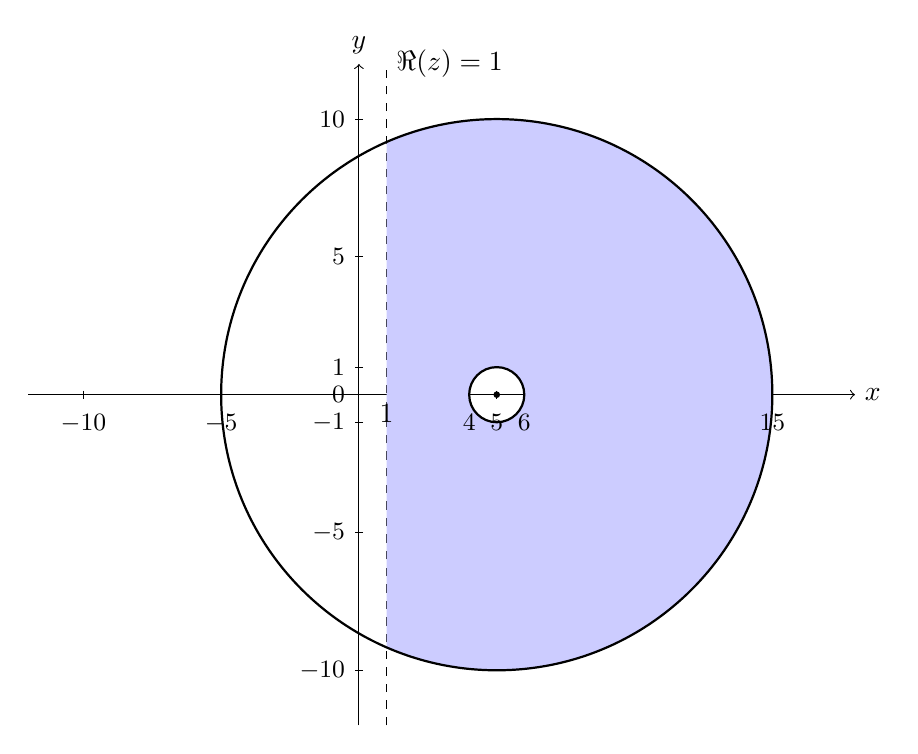
\begin{tikzpicture}[scale=0.35]
  \draw[->] (-12,0) -- (18,0) node[right] {$x$};
  \draw[->] (0,-12) -- (0,12) node[above] {$y$};

  \draw[dashed] (1,-12) -- (1,12) node[right] {$\Re(z)=1$};

  \begin{scope}
    \clip (1,-12) rectangle (18,12);
    \fill[blue!20, even odd rule] (5,0) circle (10) (5,0) circle (1);
  \end{scope}

  \draw[thick] (5,0) circle (10) node[right,yshift=-8]{};
  \draw[thick] (5,0) circle (1) node[right,yshift=-6]{};

  \fill (5,0) circle (0.12) node[below left] {};

  \node[below] at (1,0) {1};

  \foreach \x in {-10,-5,4,5,6,15}
    \draw (\x,0.15) -- (\x,-0.15) node[below,yshift=-2] {\small \(\x\)};

  \foreach \y in {-10,-5,-1,0,1,5,10}
    \draw (0.15,\y) -- (-0.15,\y) node[left,yshift=0] {\small \(\y\)};
\end{tikzpicture}


\end{document}

